%=========================================================================

\chapter{Testing} \label{chap:testing}
Most of the tests were done on 64-bit OS. The only exceptions are in performance section in \fullref{subsec:32vs64}.

For tests, multiple oprating systems were used.
\begin{itemize}
 \item RHEL 5, 64-bit - kernel 2.6.18-348.el5, gcc Red Hat 4.1.2-54
 \item RHEL 5, 32-bit - kernel 2.6.18-348.el5PAE, gcc Red Hat 4.1.2-54
 \item RHEL 7
 \item Fedora 19
\end{itemize}


\section{Functional Testing} \label{sec:functional-testing}
For the need of performance testing we wrote at first a testing application, as well as small set of scripts for automating of tests. And after getting the code on decent performance, we also used some statistical tests batteries, more information about them you can find in \fullref{sec:statistical-testing}. Later the rdrand-gen application was also created and tested, but it was already described in \fullref{chap:generator} as it is not a test application.

\TODO{Expand this chapter} % TODO expand this chapter


\section{Statistical Testing}\label{sec:statistical-testing}
Data

\TODO{TestU01 has some paper on their page - read it} % TODO TestU01 has some paper on their page - read it


\section{Performance Testing} \label{sec:performance-testing}
Because the performance of the RNG is important, we had to measure the performance. There are generaly two options of what performance can be measured:
\begin{itemize}
 \item Speed of the library
 \item Overal speed with writing the generated values
\end{itemize}
Althought during the development we measured both, here is tested primary the first option, just the library itself. 

The set of Bash and Python scripts in the {\tt tests/} directory is there for automatic run of the throughput test with different count of threads, parsing values and then creating graphs.

\TODO{measure also times for getting one number, one KiB... Don't forget to include any referenced test!} % TODO performance tests!

\subsection{32 and 64-bit difference}\label{subsec:32vs64}
A short comparison of performance on 32 and 64-bit system was made.
On machine \machine{hp-aladdin-01.lab.bos.redhat.com}, RHEL 5 was installed in both 32 and 64-bit version and the library was tested. As the figure~\ref{fig:32vs64} shows, the performance of 32-bit version is about half of 64-bit, which is exactly in expectations based on the~\fullref{sec:ISK-physical}.

\begin{figure}[h!]
  \centering
 \includegraphics[width=12cm]{fig/tests/32-64bit.eps} % Or .pdf
%\includegraphics[width=10cm,keepaspectratio]{fig/ISK-scheme}
\caption{The difference between 32 and 64-bit installation}
\label{fig:32vs64}
\end{figure}

\subsection{Half performance on some machines}

\subsection{Underflow}
The only machine on which I was able to achieve underflow of the HW RNG is \machine{dell-pr1700-02.lab.bos.redhat.com}.


\subsection{Specifications of referenced machines}
\TODO{More HW description} % TODO More HW description.

\machineDeclare{dell-pr1700-02.lab.bos.redhat.com}{Intel(R) Xeon(R) CPU E3-1285 v3 @ 3.60GHz}{The internal RNG is not able to handle more than four parallel threads at November 2013.}


\machineDeclare{hp-aladdin-01.lab.bos.redhat.com}{Intel(R) Core (TM) i7-3920XM CPU @ 2.90GHz}{HP elitebook 8770w, 4 GB RAM}



%=========================================================================